\documentclass[11pt]{article}

\usepackage[margin=1in]{geometry}
\usepackage[T1]{fontenc}
\usepackage[utf8]{inputenc}
\usepackage{lmodern}
\usepackage{microtype}
\usepackage{amsmath,amssymb,amsthm,mathtools,bm}
\usepackage{booktabs,array,longtable,tabularx}
\usepackage{enumitem}
\usepackage{xcolor}
\usepackage{hyperref}
\usepackage[most]{tcolorbox}
\usepackage{tikz}
\usepackage{pgfplots}
\usepackage{float}
\usepackage{caption}
\usepackage{fancyhdr}
\usepackage{titlesec}

\pgfplotsset{compat=1.18}
\usetikzlibrary{arrows.meta,calc,patterns,decorations.pathreplacing,positioning,backgrounds,fit,intersections}

\hypersetup{colorlinks=true,linkcolor=blue!60!black,urlcolor=blue!60!black,citecolor=blue!60!black,pdftitle={Chapter 15. Polar Coordinates and Change of Variables in the Plane}}

\setlength{\headheight}{14pt}
\setlength{\parindent}{0pt}
\setlength{\parskip}{0.65em}
\setlist[itemize]{topsep=2pt,itemsep=2pt,leftmargin=2em}
\setlist[enumerate]{topsep=2pt,itemsep=2pt,leftmargin=2em}

\titleformat{\section}{\large\bfseries}{\thesection}{0.6em}{}
\titleformat{\subsection}{\normalsize\bfseries}{\thesubsection}{0.6em}{}
\pagestyle{fancy}
\fancyhf{}
\lhead{Chapter 15. Polar Coordinates and Change of Variables}
\rhead{\thepage}
\renewcommand{\headrulewidth}{0.4pt}

\definecolor{chapterblue}{HTML}{1F5AA6}
\definecolor{chapterteal}{HTML}{168A8F}
\definecolor{chapterorange}{HTML}{D9822B}
\definecolor{chaptergreen}{HTML}{2D8A4E}
\definecolor{chapterpurple}{HTML}{6B4EAA}
\definecolor{chapterred}{HTML}{B23B3B}
\definecolor{softblue}{HTML}{EAF3FF}
\definecolor{softgreen}{HTML}{EAF8EF}
\definecolor{softorange}{HTML}{FFF4E6}
\definecolor{softpurple}{HTML}{F3EEFF}
\definecolor{softred}{HTML}{FFF0F0}
\definecolor{softgray}{HTML}{F6F7F9}

\newtcolorbox{chapteroverviewbox}{colback=softblue,colframe=chapterblue,boxrule=0.8pt,arc=2mm,left=2mm,right=2mm,top=1mm,bottom=1mm}
\newtcolorbox{goalbox}{colback=softgreen,colframe=chaptergreen,title=Learning objectives,fonttitle=\bfseries,boxrule=0.8pt,arc=2mm}
\newtcolorbox{notebox}[1][]{colback=softblue,colframe=chapterblue,title=#1,fonttitle=\bfseries,boxrule=0.7pt,arc=2mm}
\newtcolorbox{tipbox}[1][]{colback=softgreen,colframe=chaptergreen,title=#1,fonttitle=\bfseries,boxrule=0.7pt,arc=2mm}
\newtcolorbox{warningbox}[1][]{colback=softorange,colframe=chapterorange,title=#1,fonttitle=\bfseries,boxrule=0.7pt,arc=2mm}
\newtcolorbox{formulabox}[1][]{colback=softpurple,colframe=chapterpurple,title=#1,fonttitle=\bfseries,boxrule=0.8pt,arc=2mm}
\newtcbtheorem[number within=section]{workedexample}{Worked example}{enhanced,breakable,colback=white,colframe=chapterblue,colbacktitle=chapterblue,fonttitle=\bfseries,boxrule=0.7pt,arc=1.5mm,left=2mm,right=2mm,top=1mm,bottom=1mm}{ex}

\newcommand{\R}{\mathbb R}
\newcommand{\dd}{\,d}
\newcommand{\Area}{\operatorname{Area}}
\newcommand{\Jac}{\frac{\partial(x,y)}{\partial(u,v)}}

\begin{document}

\begin{center}
  {\LARGE\bfseries Chapter 15. Polar Coordinates and Change of Variables in the Plane\par}
  \vspace{0.35em}
  {\large Circular geometry, Jacobians, transformed regions, probability densities, and coordinate systems\par}
\end{center}

\begin{chapteroverviewbox}
Many two-dimensional integrals become simple only after we choose coordinates that match the geometry. Rectangular coordinates are natural for boxes and vertical slices, but circular and radial regions call for polar coordinates. More generally, a change of variables replaces a complicated region in the $xy$-plane by a simpler region in a new $uv$-plane, at the cost of multiplying by a Jacobian factor.

The central idea is
\[
\hbox{new area element}=\hbox{local area scaling factor}\times \hbox{new coordinate area element}.
\]
For polar coordinates this becomes
\[
\dd A=r\,\dd r\,\dd\theta.
\]
For a general transformation $(u,v)\mapsto (x,y)$, this becomes
\[
\dd A=\left|\frac{\partial(x,y)}{\partial(u,v)}\right|\,\dd u\,\dd v.
\]
\end{chapteroverviewbox}

\begin{goalbox}
After studying this chapter, you should be able to:
\begin{enumerate}
  \item convert between rectangular coordinates $(x,y)$ and polar coordinates $(r,\theta)$;
  \item describe disks, annuli, sectors, and shifted circles using polar inequalities;
  \item explain geometrically why $\dd A=r\,\dd r\,\dd\theta$;
  \item set up and evaluate double integrals in polar coordinates;
  \item compute and interpret the Jacobian determinant of a transformation;
  \item apply the change-of-variables formula for double integrals;
  \item connect coordinate transformations to probability densities and modern data modeling.
\end{enumerate}
\end{goalbox}

\section{Why change coordinates?}

A coordinate system is not the object itself. It is a language for describing the object. The disk
\[
x^2+y^2\le 1
\]
is simple geometrically, but in rectangular coordinates it requires square roots:
\[
-1\le x\le 1,\qquad -\sqrt{1-x^2}\le y\le \sqrt{1-x^2}.
\]
In polar coordinates, the same disk becomes
\[
0\le r\le 1,\qquad 0\le \theta\le 2\pi.
\]
The geometry did not change; only the description changed. A good coordinate system reduces complexity.

This principle appears throughout applied mathematics: ellipses become circles after scaling, correlated Gaussian densities become independent after a linear transformation, and complicated constraints may become rectangles in new variables.

\section{Polar coordinates}

In polar coordinates, a point is described by distance $r$ from the origin and angle $\theta$ from the positive $x$-axis. The conversion formulas are
\[
x=r\cos\theta,\qquad y=r\sin\theta,
\]
and
\[
r^2=x^2+y^2,\qquad \tan\theta=\frac{y}{x}
\]
when $x\ne0$, with the quadrant determining the correct angle.

\begin{figure}[H]
\centering
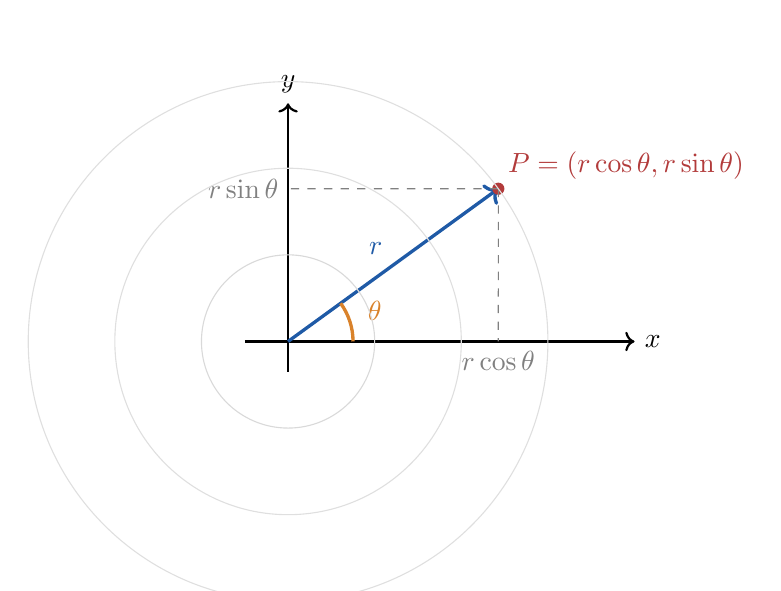
\begin{tikzpicture}[scale=1.1]
  \coordinate (O) at (0,0);
  \def\r{3.0}
  \def\ang{36}
  \coordinate (P) at ({\r*cos(\ang)},{\r*sin(\ang)});
  \draw[->,thick] (-0.5,0)--(4.0,0) node[right] {$x$};
  \draw[->,thick] (0,-0.35)--(0,2.75) node[above] {$y$};
  \draw[->,very thick,chapterblue] (O)--(P) node[midway,above left] {$r$};
  \fill[chapterred] (P) circle (2pt) node[above right] {$P=(r\cos\theta,r\sin\theta)$};
  \draw[dashed,gray] (P)--({\r*cos(\ang)},0) node[below] {$r\cos\theta$};
  \draw[dashed,gray] (P)--(0,{\r*sin(\ang)}) node[left] {$r\sin\theta$};
  \draw[chapterorange,very thick] (0.75,0) arc[start angle=0,end angle=\ang,radius=0.75];
  \node[chapterorange] at (1.0,0.35) {$\theta$};
  \draw[gray!30] (0,0) circle (1);
  \draw[gray!25] (0,0) circle (2);
  \draw[gray!25] (0,0) circle (3);
\end{tikzpicture}
\caption{A point described by polar coordinates. The radius gives distance from the origin and the angle gives direction.}
\end{figure}

\subsection*{Nonuniqueness of polar coordinates}

A rectangular coordinate pair $(x,y)$ is unique. Polar coordinates are not unique. For example, $(1,1)$ has polar coordinates
\[
\left(\sqrt2,\frac{\pi}{4}\right),\qquad
\left(\sqrt2,\frac{\pi}{4}+2\pi\right),\qquad
\left(\sqrt2,\frac{\pi}{4}+4\pi\right),
\]
and many more. The origin has $r=0$ and any value of $\theta$.

\begin{notebox}[Practical convention]
When setting up polar integrals, choose bounds so that almost every point in the region is counted exactly once. Boundaries may overlap, but overlapping boundaries have area zero and do not change a double integral.
\end{notebox}

\section{Common polar regions}

Polar coordinates are most useful when the region is described naturally by distance from the origin and angle.

\begin{center}
\begin{tabular}{@{}lll@{}}
\toprule
Region & Rectangular description & Polar description \\
\midrule
Disk & $x^2+y^2\le a^2$ & $0\le r\le a$, $0\le\theta\le2\pi$ \\
Annulus & $a^2\le x^2+y^2\le b^2$ & $a\le r\le b$, $0\le\theta\le2\pi$ \\
Sector & circular wedge & $0\le r\le a$, $\alpha\le\theta\le\beta$ \\
Upper half-disk & $x^2+y^2\le a^2$, $y\ge0$ & $0\le r\le a$, $0\le\theta\le\pi$ \\
Shifted circle & $(x-a)^2+y^2\le a^2$ & $0\le r\le2a\cos\theta$, $-\pi/2\le\theta\le\pi/2$ \\
\bottomrule
\end{tabular}
\end{center}

For the shifted circle $(x-a)^2+y^2=a^2$, expanding gives $x^2+y^2=2ax$. In polar coordinates this is $r^2=2ar\cos\theta$, so for $r\ge0$ the boundary is $r=2a\cos\theta$.

\begin{figure}[H]
\centering
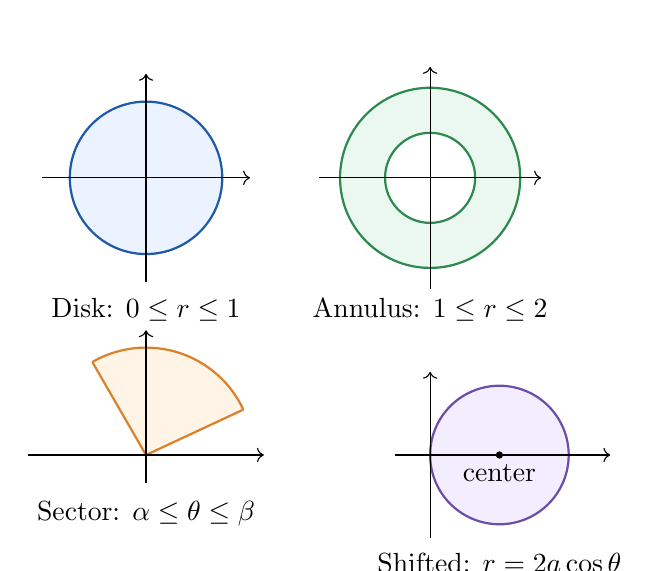
\begin{tikzpicture}[scale=0.88]
  \begin{scope}[shift={(0,0)}]
    \fill[softblue] (0,0) circle (1.1);
    \draw[chapterblue,thick] (0,0) circle (1.1);
    \draw[->] (-1.5,0)--(1.5,0); \draw[->] (0,-1.5)--(0,1.5);
    \node at (0,-1.9) {Disk: $0\le r\le1$};
  \end{scope}
  \begin{scope}[shift={(4.1,0)}]
    \fill[softgreen,even odd rule] (0,0) circle (1.3) (0,0) circle (0.65);
    \draw[chaptergreen,thick] (0,0) circle (1.3); \draw[chaptergreen,thick] (0,0) circle (0.65);
    \draw[->] (-1.6,0)--(1.6,0); \draw[->] (0,-1.6)--(0,1.6);
    \node at (0,-1.9) {Annulus: $1\le r\le2$};
  \end{scope}
  \begin{scope}[shift={(0,-4.0)}]
    \fill[softorange] (0,0)--(25:1.55) arc[start angle=25,end angle=120,radius=1.55]--cycle;
    \draw[chapterorange,thick] (25:1.55) arc[start angle=25,end angle=120,radius=1.55];
    \draw[chapterorange,thick] (0,0)--(25:1.55); \draw[chapterorange,thick] (0,0)--(120:1.55);
    \draw[->] (-1.7,0)--(1.7,0); \draw[->] (0,-0.4)--(0,1.8);
    \node at (0,-0.85) {Sector: $\alpha\le\theta\le\beta$};
  \end{scope}
  \begin{scope}[shift={(4.1,-4.0)}]
    \fill[softpurple] (0:0) plot[domain=-90:90,samples=120] ({2*cos(\x)*cos(\x)},{2*cos(\x)*sin(\x)}) -- cycle;
    \draw[chapterpurple,thick] plot[domain=-90:90,samples=120] ({2*cos(\x)*cos(\x)},{2*cos(\x)*sin(\x)});
    \draw[->] (-0.5,0)--(2.6,0); \draw[->] (0,-1.2)--(0,1.2);
    \fill (1,0) circle (1.5pt) node[below] {center};
    \node at (1,-1.55) {Shifted: $r=2a\cos\theta$};
  \end{scope}
\end{tikzpicture}
\caption{Disks, annuli, sectors, and shifted circles have compact descriptions in polar coordinates.}
\end{figure}

\section{The polar area element}

The most important formula in polar integration is
\[
\dd A=r\,\dd r\,\dd\theta.
\]
The factor $r$ is not optional. It records the fact that a small angular change $\dd\theta$ sweeps out a longer arc when the point is farther from the origin.

Consider a small polar rectangle:
\[
r\le \rho\le r+\dd r,\qquad \theta\le \phi\le \theta+\dd\theta.
\]
Its radial thickness is approximately $\dd r$. Its angular width is approximately arc length $r\,\dd\theta$. Therefore its area is approximately $(r\,\dd\theta)(\dd r)=r\,\dd r\,\dd\theta$.

\begin{figure}[H]
\centering
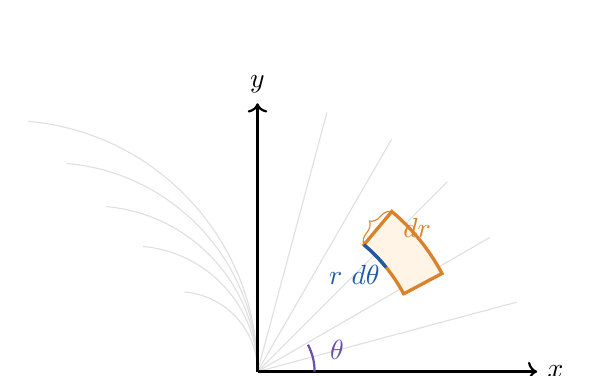
\begin{tikzpicture}[scale=1.45]
  \def\r{1.45}
  \def\dr{0.38}
  \def\a{28}
  \def\b{50}
  \foreach \rad in {0.7,1.1,1.45,1.83,2.2}{\draw[gray!25] (0,0) arc[start angle=0,end angle=85,radius=\rad];}
  \foreach \ang in {0,15,30,45,60,75}{\draw[gray!25] (0,0)--(\ang:2.35);}
  \path[fill=softorange,draw=chapterorange,very thick] (\a:\r) -- (\a:{\r+\dr}) arc[start angle=\a,end angle=\b,radius={\r+\dr}] -- (\b:\r) arc[start angle=\b,end angle=\a,radius=\r] -- cycle;
  \draw[decorate,decoration={brace,amplitude=4pt},chapterorange] (\b:\r) -- (\b:{\r+\dr}) node[midway,right=4pt] {$\dd r$};
  \draw[chapterblue,very thick] ({(\a+\b)/2}:\r) arc[start angle={(\a+\b)/2},end angle=\b,radius=\r];
  \node[chapterblue] at (45:1.20) {$r\,\dd\theta$};
  \draw[->,thick] (0,0)--(2.45,0) node[right] {$x$};
  \draw[->,thick] (0,0)--(0,2.35) node[above] {$y$};
  \draw[chapterpurple,thick] (0.5,0) arc[start angle=0,end angle=\a,radius=0.5];
  \node[chapterpurple] at (15:0.72) {$\theta$};
\end{tikzpicture}
\caption{A small polar coordinate cell has radial thickness $\dd r$ and angular width approximately $r\,\dd\theta$, so its area is approximately $r\,\dd r\,\dd\theta$.}
\end{figure}

\begin{warningbox}[Common mistake]
Do not write $\dd A=\dd r\,\dd\theta$. The correct formula is $\dd A=r\,\dd r\,\dd\theta$. The factor $r$ is the local stretching factor from angular movement.
\end{warningbox}

\section{Double integrals in polar coordinates}

Suppose a region $D$ is described in polar form as
\[
\alpha\le\theta\le\beta,\qquad h_1(\theta)\le r\le h_2(\theta).
\]
Then
\begin{formulabox}[Polar double-integral formula]
\[
\iint_D f(x,y)\,\dd A=
\int_\alpha^\beta\int_{h_1(\theta)}^{h_2(\theta)}
f(r\cos\theta,r\sin\theta)\,r\,\dd r\,\dd\theta.
\]
\end{formulabox}

The process has three steps: rewrite the region in polar bounds, substitute $x=r\cos\theta$ and $y=r\sin\theta$ into the integrand, and replace $\dd A$ by $r\,\dd r\,\dd\theta$.

\begin{workedexample}{Area of a disk}{diskarea}
Find the area of the disk $D:x^2+y^2\le a^2$.

Since $D$ is $0\le r\le a$, $0\le\theta\le2\pi$,
\[
\Area(D)=\int_0^{2\pi}\int_0^a r\,\dd r\,\dd\theta
=\int_0^{2\pi}\frac{a^2}{2}\,\dd\theta=\pi a^2.
\]
\end{workedexample}

\begin{workedexample}{Converting a rectangular-coordinate integral}{upperhalf}
Convert and evaluate
\[
\int_{-1}^{1}\int_0^{\sqrt{1-x^2}}4\,\dd y\,\dd x.
\]
The region is the upper half of the unit disk. In polar coordinates,
\[
0\le r\le1,\qquad 0\le\theta\le\pi.
\]
Therefore
\[
\int_{-1}^{1}\int_0^{\sqrt{1-x^2}}4\,\dd y\,\dd x
=\int_0^\pi\int_0^1 4r\,\dd r\,\dd\theta=2\pi.
\]
\end{workedexample}

\begin{figure}[H]
\centering
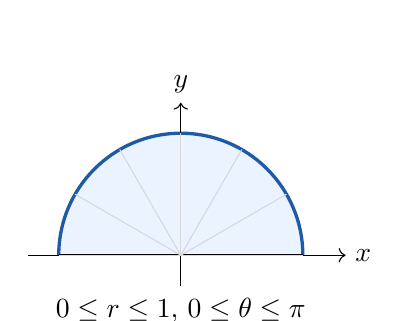
\begin{tikzpicture}[scale=1.55]
  \fill[softblue] (-1,0) arc[start angle=180,end angle=0,radius=1] -- cycle;
  \draw[chapterblue,very thick] (-1,0) arc[start angle=180,end angle=0,radius=1];
  \draw[thick] (-1,0)--(1,0);
  \draw[->] (-1.25,0)--(1.35,0) node[right] {$x$};
  \draw[->] (0,-0.25)--(0,1.25) node[above] {$y$};
  \foreach \ang in {0,30,60,90,120,150,180}{\draw[gray!30] (0,0)--(\ang:1);}
  \node at (0,-0.45) {$0\le r\le1$, $0\le\theta\le\pi$};
\end{tikzpicture}
\caption{The region for the rectangular integral is the upper half of the unit disk.}
\end{figure}

\begin{workedexample}{An annular integral}{annularintegral}
Evaluate
\[
\iint_D \cos(x^2+y^2)\,\dd A,
\]
where $D$ is the region between $r=3$ and $r=4$ in the upper half-plane.

The bounds are $3\le r\le4$ and $0\le\theta\le\pi$. Since $x^2+y^2=r^2$,
\[
\iint_D \cos(x^2+y^2)\,\dd A
=\int_0^\pi\int_3^4 \cos(r^2)r\,\dd r\,\dd\theta.
\]
Let $u=r^2$, so $\dd u=2r\,\dd r$. Then
\[
\int_3^4 \cos(r^2)r\,\dd r=\frac12\int_9^{16}\cos u\,\dd u=\frac12(\sin16-\sin9).
\]
Thus
\[
\iint_D \cos(x^2+y^2)\,\dd A=\frac{\pi}{2}(\sin16-\sin9).
\]
\end{workedexample}

\section{Volume using polar coordinates}

If a solid lies under $z=f(x,y)$ and above a region $D$, then its volume is
\[
V=\iint_D f(x,y)\,\dd A.
\]
When $D$ is circular or the function depends on $x^2+y^2$, polar coordinates often simplify the integral.

\begin{workedexample}{Paraboloid over a quadrant}{paraboloidquadrant}
Find the volume under
\[
z=6-2x^2-2y^2
\]
above the first-quadrant part of the region where $z\ge0$.

The condition $z\ge0$ gives $x^2+y^2\le3$. In the first quadrant,
\[
0\le\theta\le\frac{\pi}{2},\qquad 0\le r\le\sqrt3.
\]
Therefore
\[
V=\int_0^{\pi/2}\int_0^{\sqrt3}(6-2r^2)r\,\dd r\,\dd\theta.
\]
The inner integral is
\[
\int_0^{\sqrt3}(6r-2r^3)\,\dd r
=\left[3r^2-\frac12r^4\right]_0^{\sqrt3}=\frac92.
\]
Hence $V=\frac{\pi}{2}\cdot\frac92=\frac{9\pi}{4}$.
\end{workedexample}

\begin{figure}[H]
\centering
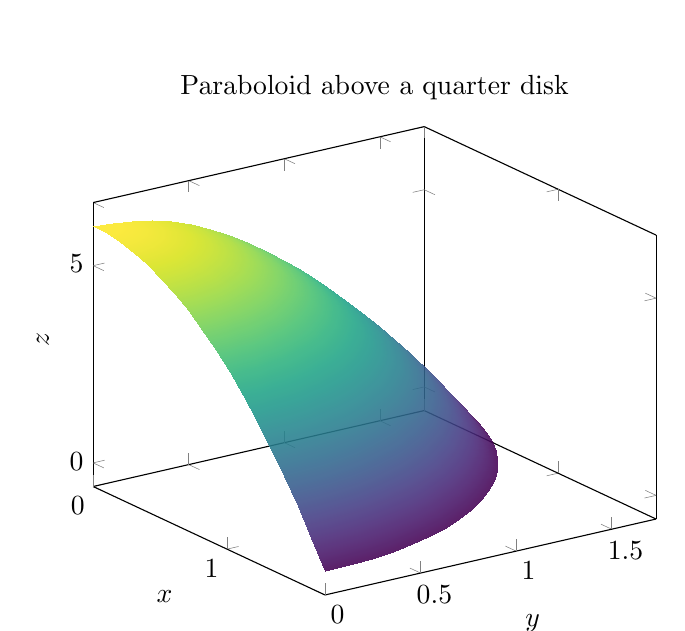
\begin{tikzpicture}
\begin{axis}[
  width=0.72\textwidth,
  view={55}{25},
  xlabel={$x$},ylabel={$y$},zlabel={$z$},
  domain=0:90, y domain=0:1.732,
  samples=22,samples y=18,
  colormap/viridis,
  z buffer=sort,
  title={Paraboloid above a quarter disk}
]
\addplot3[surf,shader=interp,opacity=0.88] ({y*cos(x)},{y*sin(x)},{6-2*y^2});
\end{axis}
\end{tikzpicture}
\caption{The surface $z=6-2x^2-2y^2$ above a quarter disk. Polar coordinates match both the circular boundary and the radial integrand.}
\end{figure}

\section{Shifted circular regions}

Polar coordinates are not only for circles centered at the origin. They also work well for some shifted circles, especially when the circle passes through the origin.

Consider
\[
D=\{(x,y):(x-2)^2+y^2\le4\}.
\]
Expanding gives $x^2+y^2\le4x$. In polar coordinates this becomes $r^2\le4r\cos\theta$, so for $r\ge0$,
\[
0\le r\le4\cos\theta,
\qquad -\frac{\pi}{2}\le\theta\le\frac{\pi}{2}.
\]
The area is
\[
\int_{-\pi/2}^{\pi/2}\int_0^{4\cos\theta}r\,\dd r\,\dd\theta
=\int_{-\pi/2}^{\pi/2}8\cos^2\theta\,\dd\theta=4\pi,
\]
which agrees with the area of a circle of radius $2$.

\begin{figure}[H]
\centering
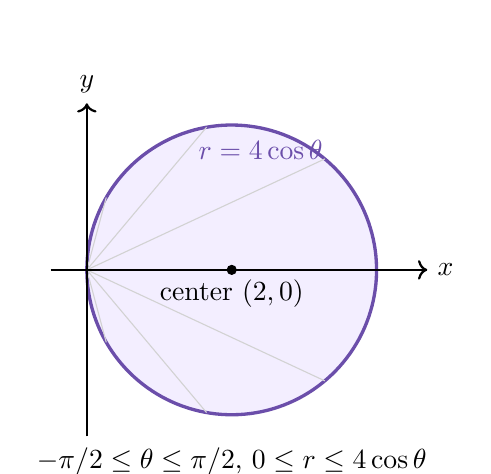
\begin{tikzpicture}[scale=0.92]
  \fill[softpurple] (0:0) plot[domain=-90:90,samples=160] ({4*cos(\x)*cos(\x)},{4*cos(\x)*sin(\x)}) -- cycle;
  \draw[chapterpurple,very thick] plot[domain=-90:90,samples=160] ({4*cos(\x)*cos(\x)},{4*cos(\x)*sin(\x)});
  \foreach \ang in {-75,-50,-25,0,25,50,75}{\draw[gray!35] (0,0)--({4*cos(\ang)*cos(\ang)},{4*cos(\ang)*sin(\ang)});}
  \draw[->,thick] (-0.5,0)--(4.7,0) node[right] {$x$};
  \draw[->,thick] (0,-2.3)--(0,2.3) node[above] {$y$};
  \fill (2,0) circle (2pt) node[below] {center $(2,0)$};
  \node[chapterpurple] at (2.4,1.65) {$r=4\cos\theta$};
  \node at (2,-2.65) {$-\pi/2\le\theta\le\pi/2$, $0\le r\le4\cos\theta$};
\end{tikzpicture}
\caption{The shifted disk $(x-2)^2+y^2\le4$ is described by $0\le r\le4\cos\theta$, $-\pi/2\le\theta\le\pi/2$.}
\end{figure}

\section{Strategy for choosing polar coordinates}

Polar coordinates are often a good choice when at least one of the following appears:
\begin{enumerate}
  \item the region involves $x^2+y^2$;
  \item the boundary is a circle, disk, annulus, sector, or ray from the origin;
  \item the integrand contains $x^2+y^2$, $\sqrt{x^2+y^2}$, or radial symmetry;
  \item a rectangular-coordinate integral contains square roots such as $\sqrt{a^2-x^2}$;
  \item the geometry is best described by distance and angle.
\end{enumerate}
Polar coordinates may not help if the region is rectangular and the integrand has no radial structure.

\begin{workedexample}{A radial integrand over a disk}{radialintegrand}
The integral
\[
\int_{-1}^{1}\int_{-\sqrt{1-x^2}}^{\sqrt{1-x^2}} e^{-(x^2+y^2)}\,\dd y\,\dd x
\]
is hard in rectangular coordinates. In polar coordinates it becomes
\[
\int_0^{2\pi}\int_0^1 e^{-r^2}r\,\dd r\,\dd\theta
=2\pi\left[-\frac12e^{-r^2}\right]_0^1=\pi(1-e^{-1}).
\]
\end{workedexample}

\begin{figure}[H]
\centering
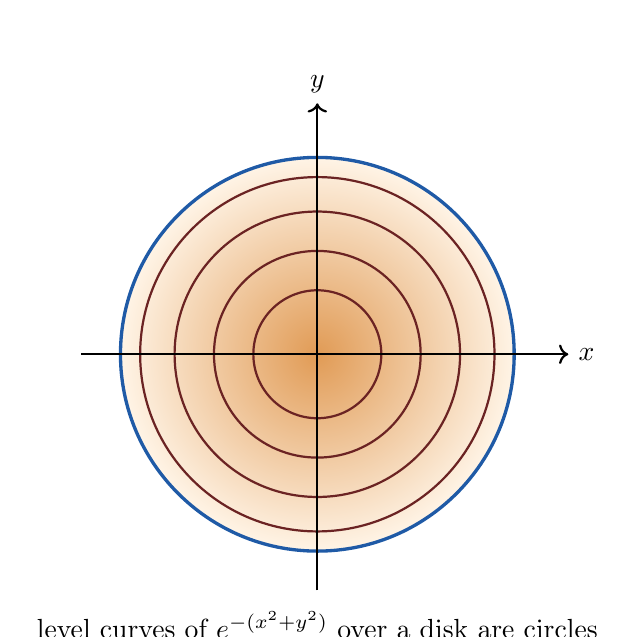
\begin{tikzpicture}[scale=1.25]
  \shade[inner color=chapterorange!80,outer color=softorange] (0,0) circle (2);
  \foreach \rad/\lab in {0.65/.7,1.05/.4,1.45/.15,1.8/.04}{\draw[chapterred!60!black,thick] (0,0) circle (\rad);}
  \draw[chapterblue,very thick] (0,0) circle (2);
  \draw[->,thick] (-2.4,0)--(2.55,0) node[right] {$x$};
  \draw[->,thick] (0,-2.4)--(0,2.55) node[above] {$y$};
  \node at (0,-2.75) {level curves of $e^{-(x^2+y^2)}$ over a disk are circles};
\end{tikzpicture}
\caption{A radially symmetric integrand over a disk. Polar coordinates turn the integral into a radial integral times an angular factor.}
\end{figure}

\section{General change of variables}

Polar coordinates are one example of a broader idea. Let a transformation $T$ map a point $(u,v)$ in a new coordinate plane to a point $(x,y)$ in the original plane:
\[
T(u,v)=(x(u,v),y(u,v)).
\]
The Jacobian determinant of the transformation is
\[
\Jac=
\begin{vmatrix}
\dfrac{\partial x}{\partial u} & \dfrac{\partial x}{\partial v} \\
\dfrac{\partial y}{\partial u} & \dfrac{\partial y}{\partial v}
\end{vmatrix}
=\frac{\partial x}{\partial u}\frac{\partial y}{\partial v}-\frac{\partial x}{\partial v}\frac{\partial y}{\partial u}.
\]
The absolute value of this determinant measures local area scaling.

\begin{formulabox}[Change-of-variables formula]
If $T$ maps a region $S$ in the $uv$-plane to a region $D$ in the $xy$-plane, and if the transformation behaves well on the region, then
\[
\iint_D f(x,y)\,\dd A
=\iint_S f(x(u,v),y(u,v))\left|\frac{\partial(x,y)}{\partial(u,v)}\right|\,\dd u\,\dd v.
\]
\end{formulabox}

For polar coordinates, $x=r\cos\theta$ and $y=r\sin\theta$. The Jacobian is
\[
\frac{\partial(x,y)}{\partial(r,\theta)}=
\begin{vmatrix}
\cos\theta & -r\sin\theta\\
\sin\theta & r\cos\theta
\end{vmatrix}=r.
\]
Thus the polar formula is just the general change-of-variables formula applied to the polar map.

\begin{figure}[H]
\centering
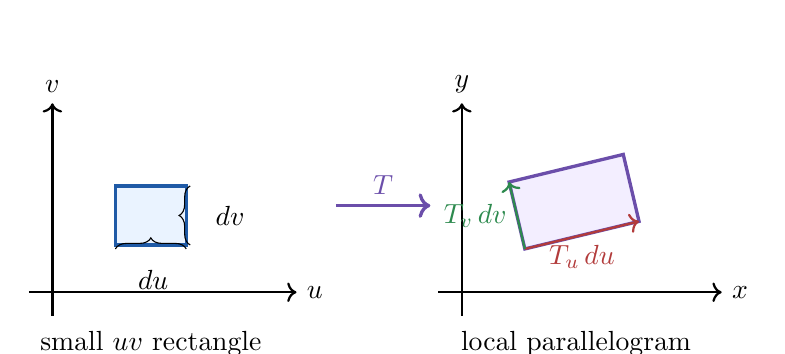
\begin{tikzpicture}[scale=1.0]
  \begin{scope}
    \draw[->,thick] (-0.3,0)--(3.1,0) node[right] {$u$};
    \draw[->,thick] (0,-0.3)--(0,2.4) node[above] {$v$};
    \fill[softblue] (0.8,0.6) rectangle (1.7,1.35);
    \draw[chapterblue,very thick] (0.8,0.6) rectangle (1.7,1.35);
    \node at (1.25,-0.65) {small $uv$ rectangle};
    \draw[decorate,decoration={brace,amplitude=4pt}] (0.8,0.55)--(1.7,0.55) node[midway,below=4pt] {$\dd u$};
    \draw[decorate,decoration={brace,amplitude=4pt}] (1.75,0.6)--(1.75,1.35) node[midway,right=4pt] {$\dd v$};
  \end{scope}
  \draw[->,very thick,chapterpurple] (3.6,1.1) -- (4.8,1.1) node[midway,above] {$T$};
  \begin{scope}[shift={(5.2,0)}]
    \draw[->,thick] (-0.3,0)--(3.3,0) node[right] {$x$};
    \draw[->,thick] (0,-0.3)--(0,2.4) node[above] {$y$};
    \coordinate (A) at (0.8,0.55); \coordinate (B) at (2.25,0.9); \coordinate (C) at (2.05,1.75); \coordinate (D) at (0.6,1.4);
    \fill[softpurple] (A)--(B)--(C)--(D)--cycle;
    \draw[chapterpurple,very thick] (A)--(B)--(C)--(D)--cycle;
    \draw[->,chapterred,thick] (A)--(B) node[midway,below] {$T_u\dd u$};
    \draw[->,chaptergreen,thick] (A)--(D) node[midway,left] {$T_v\dd v$};
    \node at (1.45,-0.65) {local parallelogram};
  \end{scope}
\end{tikzpicture}
\caption{The Jacobian determinant measures how a small coordinate rectangle is transformed into a small parallelogram in the original plane.}
\end{figure}

\section{Linear transformations and area scaling}

A linear transformation
\[
\begin{pmatrix}x\\y\end{pmatrix}=A\begin{pmatrix}u\\v\end{pmatrix}
\]
scales every area by the constant factor $|\det A|$. For example,
\[
x=2u+v,\qquad y=u+3v,
\]
so
\[
A=\begin{pmatrix}2&1\\1&3\end{pmatrix},\qquad \det A=5.
\]
Any region in the $uv$-plane has image area five times as large in the $xy$-plane.

\begin{figure}[H]
\centering
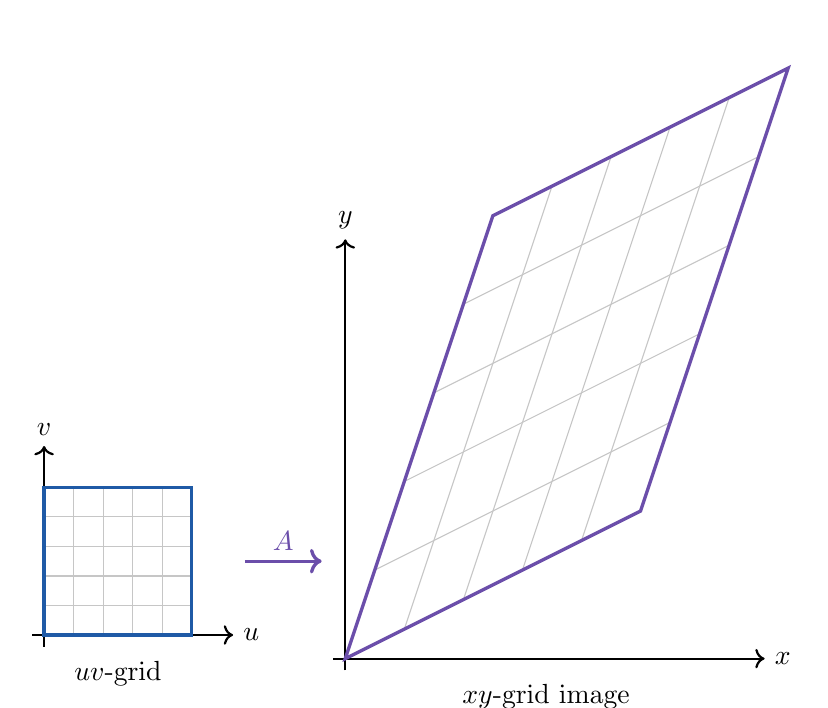
\begin{tikzpicture}[scale=0.75]
  \begin{scope}
    \draw[->,thick] (-0.2,0)--(3.2,0) node[right] {$u$};
    \draw[->,thick] (0,-0.2)--(0,3.2) node[above] {$v$};
    \foreach \c in {0,0.5,...,2.5}{\draw[gray!45] (\c,0)--(\c,2.5); \draw[gray!45] (0,\c)--(2.5,\c);}
    \draw[chapterblue,very thick] (0,0) rectangle (2.5,2.5);
    \node at (1.25,-0.65) {$uv$-grid};
  \end{scope}
  \draw[->,very thick,chapterpurple] (3.4,1.25)--(4.7,1.25) node[midway,above] {$A$};
  \begin{scope}[shift={(5.1,-0.4)}]
    \draw[->,thick] (-0.2,0)--(7.1,0) node[right] {$x$};
    \draw[->,thick] (0,-0.2)--(0,7.1) node[above] {$y$};
    \foreach \c in {0,0.5,...,2.5}{
      \draw[gray!45] ({2*\c},{\c})--({2*\c+2.5},{\c+7.5});
      \draw[gray!45] ({\c},{3*\c})--({5+\c},{2.5+3*\c});
    }
    \draw[chapterpurple,very thick] (0,0)--(5,2.5)--(7.5,10)--(2.5,7.5)--cycle;
    \node at (3.4,-0.65) {$xy$-grid image};
  \end{scope}
\end{tikzpicture}
\caption{A square grid in the $uv$-plane transformed by a linear map. The determinant gives the constant area-scaling factor.}
\end{figure}

\begin{workedexample}{Area of a parallelogram}{parallelogramarea}
Let $S=[0,1]\times[0,1]$ and define
\[
x=2u+v,\qquad y=u+3v.
\]
The image $D=T(S)$ is a parallelogram. Since $|\det A|=5$,
\[
\Area(D)=\iint_D1\,\dd A=\iint_S 1\cdot5\,\dd u\,\dd v=5.
\]
\end{workedexample}

\section{Nonlinear transformations}

For nonlinear transformations, the Jacobian usually varies from point to point. The transformation may stretch one part of the region more than another.

For example,
\[
x=u,\qquad y=v+0.4u^2.
\]
The Jacobian is
\[
\frac{\partial(x,y)}{\partial(u,v)}=\begin{vmatrix}1&0\\0.8u&1\end{vmatrix}=1.
\]
Although this transformation bends horizontal grid lines into parabolas, it preserves area locally because the Jacobian determinant is $1$.

\begin{figure}[H]
\centering
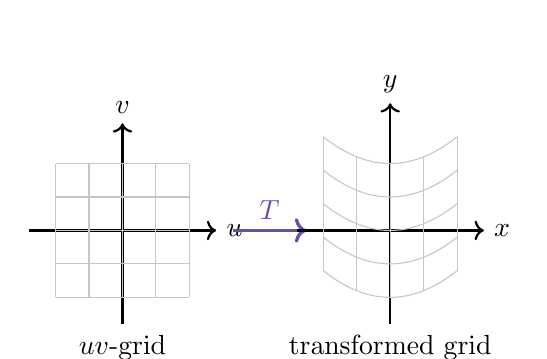
\begin{tikzpicture}[scale=0.85]
  \begin{scope}
    \draw[->,thick] (-1.4,0)--(1.4,0) node[right] {$u$};
    \draw[->,thick] (0,-1.4)--(0,1.6) node[above] {$v$};
    \foreach \c in {-1,-0.5,...,1}{\draw[gray!45] (\c,-1)--(\c,1); \draw[gray!45] (-1,\c)--(1,\c);}
    \node at (0,-1.75) {$uv$-grid};
  \end{scope}
  \draw[->,very thick,chapterpurple] (1.65,0)--(2.75,0) node[midway,above] {$T$};
  \begin{scope}[shift={(4.0,0)}]
    \draw[->,thick] (-1.4,0)--(1.4,0) node[right] {$x$};
    \draw[->,thick] (0,-1.4)--(0,1.9) node[above] {$y$};
    \foreach \c in {-1,-0.5,...,1}{
      \draw[gray!45] (\c,{-1+0.4*\c*\c})--(\c,{1+0.4*\c*\c});
      \draw[gray!45,domain=-1:1,samples=40] plot (\x,{\c+0.4*\x*\x});
    }
    \node at (0,-1.75) {transformed grid};
  \end{scope}
\end{tikzpicture}
\caption{A nonlinear shear bends grid lines but has Jacobian determinant $1$, so it preserves area locally.}
\end{figure}

\begin{workedexample}{A triangular transformation}{triangular}
Let
\[
x=u,
\qquad y=uv,
\qquad 1\le u\le2,
\qquad 0\le v\le1.
\]
The Jacobian is
\[
\frac{\partial(x,y)}{\partial(u,v)}=
\begin{vmatrix}1&0\\v&u\end{vmatrix}=u.
\]
The image region satisfies $1\le x\le2$ and $0\le y\le x$. Hence
\[
\iint_D(x+y)\,\dd A=\int_1^2\int_0^1 (u+uv)u\,\dd v\,\dd u
=\int_1^2\frac32u^2\,\dd u=\frac72.
\]
\end{workedexample}

\section{Change of variables in probability}

Change of variables is essential in probability and statistics. If $(X,Y)$ has joint density $f_{X,Y}(x,y)$ and $(X,Y)=T(U,V)$, then the density of $(U,V)$ involves a Jacobian factor. Informally,
\[
\hbox{probability mass}=\hbox{density}\times\hbox{area}.
\]
When area changes, density must change in the opposite way so that probability is preserved.

\subsection*{Radial probability}
Suppose a density depends only on radius:
\[
f(x,y)=c e^{-(x^2+y^2)}.
\]
To find the normalizing constant $c$, require
\[
1=\iint_{\R^2}c e^{-(x^2+y^2)}\,\dd A.
\]
Using polar coordinates,
\[
1=c\int_0^{2\pi}\int_0^\infty e^{-r^2}r\,\dd r\,\dd\theta
=c(2\pi)\left(\frac12\right)=c\pi.
\]
Thus $c=1/\pi$.

\begin{figure}[H]
\centering
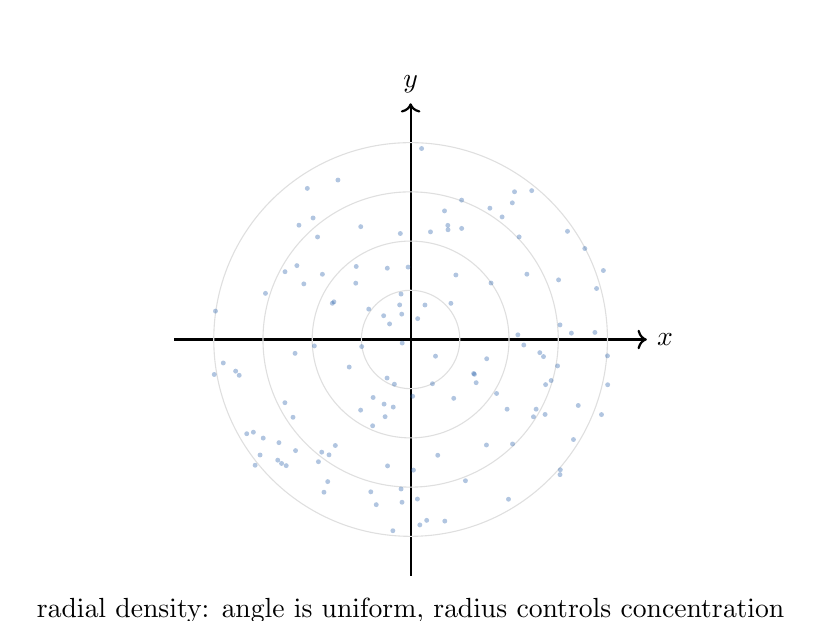
\begin{tikzpicture}[scale=1.25]
  \draw[->,thick] (-2.4,0)--(2.4,0) node[right] {$x$};
  \draw[->,thick] (0,-2.4)--(0,2.4) node[above] {$y$};
  \foreach \rad in {0.5,1,1.5,2}{\draw[gray!25] (0,0) circle (\rad);}
  \foreach \i in {1,...,130}{
    \pgfmathsetmacro{\rad}{2.1*sqrt(rnd)}
    \pgfmathsetmacro{\ang}{360*rnd}
    \fill[chapterblue,opacity=0.35] ({\rad*cos(\ang)},{\rad*sin(\ang)}) circle (0.025);
  }
  \node at (0,-2.75) {radial density: angle is uniform, radius controls concentration};
\end{tikzpicture}
\caption{Samples from a radial distribution. Polar coordinates separate radius and angle, which is useful for simulation and probability calculations.}
\end{figure}

\section{Computational viewpoint}

In computation, a change of variables is more than a symbolic trick. It is a method for transforming a difficult numerical problem into an easier one.

To approximate
\[
\iint_{x^2+y^2\le1}e^{-(x^2+y^2)}\,\dd A,
\]
we can sample uniformly from the disk. A correct polar simulation must not sample $r$ uniformly on $[0,1]$. Since area in polar coordinates is $r\,\dd r\,\dd\theta$, the radius distribution must put more points near the outer part of the disk.

A uniform point in the unit disk can be generated by
\[
\Theta\sim\operatorname{Uniform}(0,2\pi),\qquad R=\sqrt U,
\]
where $U\sim\operatorname{Uniform}(0,1)$.

\begin{figure}[H]
\centering
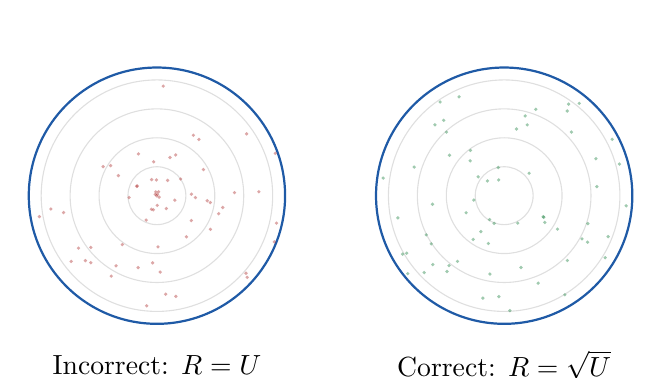
\begin{tikzpicture}[scale=1.05]
  \begin{scope}
    \draw[chapterblue,thick] (0,0) circle (1.55);
    \foreach \rad in {0.35,0.7,1.05,1.4}{\draw[gray!25] (0,0) circle (\rad);}
    \foreach \k in {1,...,65}{\pgfmathsetmacro{\rad}{1.55*rnd}\pgfmathsetmacro{\ang}{360*rnd}\fill[chapterred,opacity=0.45] ({\rad*cos(\ang)},{\rad*sin(\ang)}) circle (0.022);}
    \node at (0,-2.05) {Incorrect: $R=U$};
  \end{scope}
  \begin{scope}[shift={(4.2,0)}]
    \draw[chapterblue,thick] (0,0) circle (1.55);
    \foreach \rad in {0.35,0.7,1.05,1.4}{\draw[gray!25] (0,0) circle (\rad);}
    \foreach \k in {1,...,65}{\pgfmathsetmacro{\rad}{1.55*sqrt(rnd)}\pgfmathsetmacro{\ang}{360*rnd}\fill[chaptergreen,opacity=0.45] ({\rad*cos(\ang)},{\rad*sin(\ang)}) circle (0.022);}
    \node at (0,-2.05) {Correct: $R=\sqrt U$};
  \end{scope}
\end{tikzpicture}
\caption{Uniform sampling in a disk requires $R=\sqrt U$, not $R=U$. The Jacobian factor $r$ explains the difference.}
\end{figure}

The exact value of the disk integral is
\[
\int_0^{2\pi}\int_0^1 e^{-r^2}r\,\dd r\,\dd\theta=\pi(1-e^{-1}).
\]

\section{Applications in data, statistics, and AI}

\subsection*{Radial basis functions}
Many machine-learning models use radial basis functions such as
\[
\phi(x,y)=e^{-\gamma(x^2+y^2)}.
\]
These functions are constant on circles centered at the origin. Polar coordinates reveal their radial structure immediately.

\subsection*{Gaussian models}
The bivariate normal density has elliptical level curves. After shifting, scaling, and rotating coordinates, those ellipses become circles. This is a change-of-variables idea. The determinant of the covariance matrix controls how volume changes.

\subsection*{Normalizing flows}
In modern generative modeling, a normalizing flow transforms a simple latent variable $z$ into a more complicated observed variable $x=T(z)$. The probability density changes by a Jacobian determinant. In two dimensions the formula is the same idea as this chapter; in high dimensions it becomes
\[
\hbox{density correction}=|\det J_T|^{-1}.
\]

\subsection*{Numerical integration}
Monte Carlo methods, importance sampling, and coordinate transformations all rely on understanding how area or volume changes under a transformation. A poor coordinate system can make an integral numerically unstable; a good one can make the same problem nearly one-dimensional.

\section{Chapter summary}

The key polar formulas are
\[
x=r\cos\theta,\qquad y=r\sin\theta,\qquad r^2=x^2+y^2.
\]
The polar area element is
\[
\dd A=r\,\dd r\,\dd\theta.
\]
Thus, for a polar region
\[
D=\{(r,\theta):\alpha\le\theta\le\beta,\; h_1(\theta)\le r\le h_2(\theta)\},
\]
we have
\[
\iint_D f(x,y)\,\dd A
=\int_\alpha^\beta\int_{h_1(\theta)}^{h_2(\theta)} f(r\cos\theta,r\sin\theta)r\,\dd r\,\dd\theta.
\]
For a general transformation $T(u,v)=(x(u,v),y(u,v))$, the Jacobian determinant is
\[
\Jac=\begin{vmatrix}x_u&x_v\\y_u&y_v\end{vmatrix},
\]
and the change-of-variables formula is
\[
\iint_D f(x,y)\,\dd A
=\iint_S f(x(u,v),y(u,v))\left|\Jac\right|\,\dd u\,\dd v.
\]
The absolute value of the Jacobian determinant is the local area-scaling factor.

\section{Exercises}

\subsection*{Conceptual questions}
\begin{enumerate}
  \item Explain why polar coordinates are useful for disks and annuli.
  \item Explain why the polar area element is $r\,\dd r\,\dd\theta$, not $\dd r\,\dd\theta$.
  \item Why are polar coordinates not unique?
  \item What does the Jacobian determinant measure geometrically?
  \item Why do we use the absolute value of the Jacobian determinant in the change-of-variables formula?
  \item Give an example of a region where rectangular coordinates are more convenient than polar coordinates.
  \item Give an example of an integrand where polar coordinates simplify the algebra.
  \item Explain why uniform sampling in a disk requires $R=\sqrt U$ instead of $R=U$.
\end{enumerate}

\subsection*{Polar coordinate descriptions}
\begin{enumerate}[start=9]
  \item Describe the disk $x^2+y^2\le9$ in polar coordinates.
  \item Describe the annulus $4\le x^2+y^2\le25$ in polar coordinates.
  \item Describe the upper half of the disk $x^2+y^2\le16$ in polar coordinates.
  \item Describe the first-quadrant part of the annulus $1\le x^2+y^2\le4$ in polar coordinates.
  \item Convert the circle $x^2+y^2=6x$ to polar form.
  \item Convert the circle $x^2+y^2=-4y$ to polar form.
  \item Describe the region inside $r=2\cos\theta$.
  \item Describe the region inside $r=3\sin\theta$.
\end{enumerate}

\subsection*{Polar integrals}
\begin{enumerate}[start=17]
  \item Evaluate $\iint_D1\,\dd A$ where $D$ is the disk $x^2+y^2\le4$.
  \item Evaluate $\iint_D(x^2+y^2)\,\dd A$ where $D$ is the disk $x^2+y^2\le1$.
  \item Evaluate $\iint_De^{-(x^2+y^2)}\,\dd A$ where $D$ is the disk $x^2+y^2\le4$.
  \item Evaluate $\iint_D\sqrt{x^2+y^2}\,\dd A$ where $D$ is the annulus $1\le x^2+y^2\le9$.
  \item Evaluate $\iint_D y\,\dd A$ where $D$ is the upper half of the disk $x^2+y^2\le1$.
  \item Evaluate $\iint_D x^2\,\dd A$ where $D$ is the first-quadrant unit disk.
  \item Convert $\int_{-2}^2\int_0^{\sqrt{4-x^2}}f(x,y)\,\dd y\,\dd x$ to polar form.
  \item Convert $\int_0^2\int_0^{\sqrt{4-y^2}}f(x,y)\,\dd x\,\dd y$ to polar form.
  \item Evaluate the volume under $z=9-x^2-y^2$ above the disk $x^2+y^2\le9$.
  \item Evaluate the volume under $z=4-x^2-y^2$ above the first-quadrant part of $x^2+y^2\le4$.
\end{enumerate}

\subsection*{Change of variables}
\begin{enumerate}[start=27]
  \item Compute the Jacobian for $x=3u$, $y=2v$.
  \item Compute the Jacobian for $x=u+v$, $y=u-v$.
  \item Compute the Jacobian for $x=u^2-v^2$, $y=2uv$.
  \item Compute the Jacobian for $x=e^u\cos v$, $y=e^u\sin v$.
  \item Let $x=2u+v$, $y=u+4v$, and $S=[0,1]\times[0,2]$. Find the area of $T(S)$.
  \item Let $x=u$, $y=uv$, where $1\le u\le3$ and $0\le v\le2$. Write the corresponding region in the $xy$-plane.
  \item Use the change of variables $x=2u$, $y=3v$ to compute the area of the ellipse $x^2/4+y^2/9\le1$.
  \item Use an appropriate change of variables to convert the ellipse $x^2/a^2+y^2/b^2\le1$ into a unit disk.
\end{enumerate}

\subsection*{Applications and computation}
\begin{enumerate}[start=35]
  \item Use polar coordinates to normalize the density $f(x,y)=ce^{-(x^2+y^2)}$ over the plane.
  \item Find the probability that a point with density $f(x,y)=\pi^{-1}e^{-(x^2+y^2)}$ lies inside the unit disk.
  \item Write code to approximate $\iint_{x^2+y^2\le1}\sqrt{x^2+y^2}\,\dd A$ by Monte Carlo simulation.
  \item Explain how the determinant appears in a two-dimensional normalizing flow.
  \item Let $L(a,b)=\iint_D(a+br-y)^2\,\dd A$ over a disk $D$. Explain why polar coordinates may simplify the geometry but not necessarily the integrand.
  \item A sensor has circular range $x^2+y^2\le R^2$. Write an integral for the average signal strength $S(x,y)=e^{-\lambda\sqrt{x^2+y^2}}$ over the range.
\end{enumerate}

\section{Python lab and looking ahead}

In the companion Python lab, students plot polar grids and polar regions, convert rectangular integrals over disks into polar form, compute polar integrals numerically, visualize the polar area element, compute Jacobians of transformations, transform grids under linear and nonlinear maps, simulate uniform points in disks, and estimate radial probability integrals using Monte Carlo methods.

This chapter introduced coordinate transformations in the plane. The next chapters extend the same idea to three-dimensional integration. Cylindrical and spherical coordinates play the role that polar coordinates played here, and the Jacobian factors become volume-scaling factors.

\end{document}
